\documentclass{article}

\usepackage{microtype}
\usepackage{graphicx}
\usepackage{subfigure}
\usepackage{booktabs}
\usepackage{hyperref}
\usepackage{amsmath}
\usepackage{amssymb}
\usepackage{mathtools}
\usepackage{amsthm}
\usepackage[capitalize,noabbrev]{cleveref}
\usepackage{enumitem}

\newcommand{\theHalgorithm}{\arabic{algorithm}}
\usepackage[accepted]{icml2024}

\theoremstyle{plain}
\newtheorem{theorem}{Theorem}[section]
\newtheorem{proposition}[theorem]{Proposition}

\icmltitlerunning{Language-Routed Specialist Ensembles for Bilingual Sentiment}

\begin{document}

\twocolumn[
\icmltitle{Language-Routed Specialist Ensembles for \\
           Bilingual Ordinal Sentiment Classification}

\icmlsetsymbol{equal}{*}
\begin{icmlauthorlist}
\icmlauthor{Ismail Lataoui}{equal,eth}
\icmlauthor{Mehdi Hamirifou}{equal,eth}
\icmlauthor{Abdellah Janati Idrissi}{equal,eth}
\end{icmlauthorlist}
\icmlaffiliation{eth}{Department of Computer Science, ETH Zurich, Switzerland}
\icmlkeywords{sentiment classification, ordinal regression, multilingual NLP,
              ensemble learning, mixture of experts}

\vskip 0.3in
]

\printAffiliationsAndNotice{\icmlEqualContribution}

\begin{abstract}
We address bilingual ordinal sentiment classification of product reviews,
scored by mean absolute error (MAE). Two structural properties drive our
design. First, the task is ordinal: the MAE-optimal point predictor is
the \emph{median} of the predictive distribution, so we decode every
model with the median rule. Second, the corpus is bilingual at near-equal
proportions: we augment a multilingual transformer ensemble with two
\emph{monolingual specialist} encoders (DeBERTa-v3-large for English,
gBERT-large for German) and ensemble them through a metric-aware
meta-learner that fits \emph{separate} per-language simplex weights. The
final system reaches a public-leaderboard score of $\mathbf{0.911}$,
above the grade-6 baseline ($0.906$), and places second out of 27 teams.
\end{abstract}

% =================================================================
\section{Introduction}
\label{sec:intro}
% =================================================================

Star-rating prediction is a long-studied sentiment-analysis task, but the
present setting combines three properties that together make it
non-trivial. First, the corpus is \emph{bilingual} with reviews split
roughly $52/48$ between English and German, so a monolingual model
forfeits about half the data. Second, predictions are scored by mean
absolute error on a five-point scale; the task is therefore
\emph{ordinal}---confusing a one-star review with a five-star one is four
times as costly as confusing it with a two-star one. Third, the text is
\emph{noisy}: it contains typos, emojis, repeated characters
(e.g.\ \textit{sooooo}), sarcasm, and reviews whose body contradicts
their title.

The standard answer to whether the bilingual structure matters is no:
a single multilingual transformer is trained on both halves and
produces one prediction per review. We argue otherwise. Our
contributions are:
\begin{itemize}[leftmargin=*,topsep=2pt,itemsep=0pt]
\item A formal derivation of the median-decoding rule as the Bayes
predictor under MAE on integer ordinal labels
(Proposition~\ref{prop:median}), applied uniformly across all models.
\item Two \emph{monolingual specialist} encoders---DeBERTa-v3-large
\cite{he2023debertav3} on the English partition and gBERT-large
\cite{chan2020gbert} on the German partition---added to a pool of six
classical baselines and two multilingual transformers.
\item A \emph{per-language} weighted-MAE meta-learner fitting two
simplex weight vectors $w_{\mathrm{en}},w_{\mathrm{de}}\in\Delta^{K-1}$
directly minimising MAE after median decoding; at inference the
detected language selects the active weight vector.
\item A controlled comparison of six aggregators (uniform, global and
per-language weighted-MAE, stacked LogReg, stacked GBM, gating MLP)
isolating the contribution of metric-aware optimisation and
language-conditioned routing.
\end{itemize}
The final system reaches $0.911$ on the public Kaggle leaderboard
(rank $2/27$), $+0.005$ above the grade-6 baseline.

% =================================================================
\section{Data and Evaluation}
\label{sec:data}
% =================================================================

The training set contains $n_{\text{train}}=252{,}000$ labelled reviews
and the test set $n_{\text{test}}=168{,}000$. Class labels in
$\{0,\dots,4\}$ are \emph{exactly balanced} at $50{,}400$ each. All
model selection uses a single $10\%$ stratified hold-out (seed $42$,
$25{,}200$ reviews); we never tune on the public leaderboard.

\paragraph{Bilingual composition.}
A lightweight rule (umlaut
$\{\text{\"a},\text{\"o},\text{\"u},\text{ss}\}$ or any of a short
list of common German function words) assigns the labels $52\%$
\textsc{en} / $48\%$ \textsc{de}, uniform across the five rating
classes (within $\pm 2$ percentage points). We use the same detector
at training time (to partition the train set for the specialists,
\cref{sec:specialists}) and at inference time (to route in the
language-aware meta-learner, \cref{sec:meta}).

\paragraph{Surface cues.}
The ``\texttt{!}'' frequency is \emph{U-shaped} in the rating, peaking
at both one-star and five-star reviews (\cref{fig:surface}); a model
that treats it as a polarity feature confuses the two extremes---the
worst mistake under MAE. The ``\texttt{?}'' frequency, in contrast,
decreases monotonically with the rating. We use these as sanity
checks on representations, not as features.

\paragraph{Length.}
Reviews are a short title followed by a body; the $99$th percentile
is $161$ words (\cref{fig:length}). Transformer fine-tunes use
$\text{max\_length}\in\{192,256\}$, covering $\!>\!99\%$ of inputs.

\begin{figure}[t]
\centering
\subfigure[Surface cues by label.\label{fig:surface}]{
  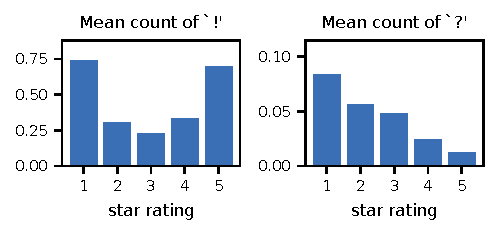
\includegraphics[width=0.46\linewidth]{figs/surface_features}}
\hfill
\subfigure[Length distribution.\label{fig:length}]{
  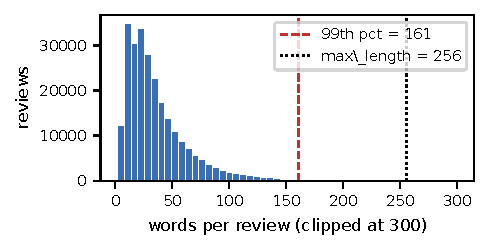
\includegraphics[width=0.46\linewidth]{figs/length_hist}}
\caption{Dataset characteristics that motivate two design choices:
the U-shape of ``\texttt{!}'' justifies context-aware representations,
and the $99$th-percentile length of $161$ words justifies
$\text{max\_length}=256$.}
\end{figure}

\paragraph{Evaluation metric.}
Predictions $\hat{\mathbf y}\in\{0,\dots,4\}^n$ are scored by
\begin{equation}
\label{eq:score}
L(\hat{\mathbf y},\mathbf y)
= 1-\frac{1}{4n}\sum_{i=1}^n |y_i-\hat y_i|
= 1-\frac{\mathrm{MAE}}{4}.
\end{equation}
Severe misclassifications ($0\!\leftrightarrow\!4$) are penalised in
proportion to their ordinal magnitude. This affine relation with MAE is
the only property we exploit in \cref{sec:decoding}: the entire
decoding-and-ensembling pipeline is derived from it.

% =================================================================
\section{Method}
\label{sec:method}
% =================================================================

\subsection{MAE-Optimal Decoding via the Median}
\label{sec:decoding}

Each of our $K$ models returns, for every review, a probability
vector $p=(p_0,\dots,p_4)$ on the five ratings. A \emph{decoding rule}
maps $p$ to an integer prediction $\hat y\in\{0,\dots,4\}$. The
standard choice $\arg\max p$ is Bayes-optimal under $0/1$ loss; under
absolute-error loss the Bayes rule is different.

\begin{proposition}\label{prop:median}
For an integer-valued $Y\in\{0,\dots,K\}$ with distribution $p$, the
constant prediction minimising $\mathbb E_Y[|Y-\hat y|]$ is the
\emph{median} $\hat y^\star=\min\{k:\sum_{j\le k}p_j\ge \tfrac{1}{2}\}$.
\end{proposition}

\begin{proof}[Sketch]
$\hat y\mapsto \mathbb E_Y[|Y-\hat y|]$ is piecewise-linear and convex;
its left/right subgradients at $\hat y=k$ are $1-2\sum_{j\le k-1}p_j$
and $1-2\sum_{j\le k}p_j$, so $k$ is optimal iff both bracket zero,
which is the median condition \citep{koltchinskii1997median}.
\end{proof}

Since~\eqref{eq:score} is affine in MAE, we decode \emph{every} model
with the median rule. The rule needs no retraining; it accepts a
slightly lower exact-match rate in exchange for fewer large errors.
Empirically, switching from $\arg\max$ to the median lifts the
validation score of every fine-tuned encoder by between $0.0003$ and
$0.0013$, and of the linear baselines by $+0.0055$ to $+0.0067$ (see
\texttt{verify\_decoding.py}).

\subsection{Base Models and Bilingual Specialists}
\label{sec:specialists}

We use six \emph{baselines} of increasing representational richness:
\textbf{B1} TF--IDF unigrams+bigrams ($50$k features) with logistic
regression; \textbf{B2} a frozen multilingual sentence encoder
(paraphrase-multilingual-MiniLM-L12, \citealt{reimers2019sbert}) with
logistic regression; \textbf{B3} a Kim-style CNN \cite{kim2014cnn};
\textbf{B4} a bidirectional LSTM \cite{hochreiter1997lstm};
\textbf{B5} gradient boosting on TruncatedSVD of TF--IDF; and
\textbf{B6} gradient boosting on $19$ hand-crafted surface features
(length, punctuation counts, capitals, emoji counts, umlaut
indicator).

Two \emph{multilingual transformers} are then fine-tuned end-to-end on
the entire $227$K-review training pool: \textbf{XLM-RoBERTa-base}
\cite{conneau2020xlmr} ($278$M parameters) and
\textbf{mDeBERTa-v3-base} \cite{he2023debertav3} ($279$M parameters),
both with a five-way classification head, AdamW
\cite{loshchilov2019adamw} ($\eta{=}2\!\times\!10^{-5}$, weight decay
$0.01$, warm-up $6\%$ of steps), $3$ epochs, batch size $16$, mixed
precision.

To the eight models above we add the two \emph{monolingual specialists}
that motivate this paper: \textbf{DeBERTa-v3-large}
\cite{he2023debertav3} ($435$M parameters, English-only pre-training)
fine-tuned on the $116{,}929$ English reviews of the training pool;
and \textbf{gBERT-large} \cite{chan2020gbert} ($336$M parameters,
German-only) on the $109{,}871$ German reviews. Both use
$\text{max\_length}{=}192$, $\eta{=}10^{-5}$, warm-up $10\%$, gradient
checkpointing (to fit a $24$-layer model on $11$\,GB), and two epochs.

\subsection{Per-Language Weighted-MAE Meta-Learner}
\label{sec:meta}

Let $\mathcal M=\{1,\dots,K\}$ be the index set of our $K{=}10$ trained
models, and write $p^{(k)}_i\in\Delta^4$ for model $k$'s posterior on
review $i$. We compare six aggregation rules; all decode with the
median.

\paragraph{Uniform / global / classical stacking.}
The simplest aggregator averages with uniform weights
$\bar p_i=\tfrac{1}{K}\sum_k p^{(k)}_i$. A first improvement is
\emph{weighted MAE}, which searches the simplex
$\Delta^{K-1}=\{w:w_k\ge 0,\sum_k w_k=1\}$ for the global weight vector
that minimises
$\sum_i \bigl|y_i-\mathrm{med}\bigl(\sum_k w_k\, p^{(k)}_i\bigr)\bigr|$
on validation; since the median is non-differentiable in $w$, we run
Dirichlet sampling followed by coordinate refinement.
We also include two standard stacked classifiers
\cite{wolpert1992stacked}: an $\ell_2$-regularised multinomial
\emph{LogReg} on the $5K$ concatenated probabilities, and a histogram
gradient-boosted classifier (\emph{GBM}, \citealt{ke2017lightgbm}).

\paragraph{Per-language weighted-MAE.}
Our central proposal exploits the bilingual structure. Let
$\ell(i)\in\{\textsc{en},\textsc{de}\}$ be the language of review $i$.
We fit two independent weight vectors,
\begin{align*}
w_{\mathrm{en}}&=\arg\min_{w\in\Delta^{K-1}}\!\!\sum_{i:\,\ell(i)=\textsc{en}}\!\!
   \bigl|y_i-\mathrm{med}\bigl(\textstyle\sum_k w_k\, p^{(k)}_i\bigr)\bigr|, \\
w_{\mathrm{de}}&=\arg\min_{w\in\Delta^{K-1}}\!\!\sum_{i:\,\ell(i)=\textsc{de}}\!\!
   \bigl|y_i-\mathrm{med}\bigl(\textstyle\sum_k w_k\, p^{(k)}_i\bigr)\bigr|.
\end{align*}
At test time, sample $i$ is routed to $w_{\ell(i)}$ via the same
detector. This is a hard-routing mixture of experts
\cite{jacobs1991moe} with two distinguishing features: (i) the routing
variable is observed, not learnt, and (ii) each expert's parameter is
a probability simplex tuned for the metric, not a neural classifier
tuned for log-loss.

\paragraph{Gating MLP.}
For comparison, a soft-routing variant: a small MLP ($384$-d MiniLM
sentence embedding + $10$ per-model max-probs + $10$ entropies + $1$
language flag $\to 64\to K$) outputs per-sample weights, trained with
a Wasserstein-1 ordinal loss and averaged over three random seeds.

\paragraph{Evaluation protocol.}
Every meta-learner is scored by $5$-fold stratified CV on the hold-out
set, producing out-of-fold (OOF) predictions on the $25{,}200$
reviews; the test submission re-fits on the full hold-out.

% =================================================================
\section{Results}
\label{sec:results}
% =================================================================

\subsection{Per-Model Performance}
\label{sec:per-model}

\cref{tab:per-model} lists every model's validation score, the per-
language breakdown, and (where submitted) the public-leaderboard score.
Three observations drive the rest of the analysis.

\begin{table}[t]
\caption{Per-model performance on the $10\%$ validation hold-out
(median decoding) and on the Kaggle public leaderboard (45\% of test).
EN/DE columns evaluate on the $12{,}871$/$12{,}329$ reviews of each
language; ``--'' marks models not submitted individually.}
\label{tab:per-model}
\vskip 0.06in
\begin{center}\begin{small}\begin{tabular}{lcccc}
\toprule
Model & Val & EN & DE & Public LB \\
\midrule
\multicolumn{5}{l}{\emph{Classical and shallow baselines}}\\
B1: TF--IDF + LogReg            & 0.882 & 0.886 & 0.879 & 0.881 \\
B2: Frozen MiniLM + LogReg      & 0.863 & 0.869 & 0.857 & 0.861 \\
B3: CNN (Kim-style, 15M)        & 0.878 & 0.880 & 0.875 & 0.877 \\
B4: BiLSTM (15M)                & 0.887 & 0.888 & 0.887 & 0.887 \\
B5: GBM on TF--IDF$+$SVD        & 0.850 & 0.856 & 0.844 & 0.851 \\
B6: GBM on surface features     & 0.722 & 0.721 & 0.724 & 0.721 \\
\midrule
\multicolumn{5}{l}{\emph{Multilingual transformers}}\\
XLM-R-base ($278$M)             & 0.905 & 0.907 & 0.903 & 0.904 \\
mDeBERTa-v3-base ($279$M)       & 0.907 & 0.909 & 0.906 & 0.906 \\
\midrule
\multicolumn{5}{l}{\emph{Monolingual specialists (this work)}}\\
DeBERTa-v3-large EN ($435$M)    & 0.908 & \textbf{0.914} & 0.902 & -- \\
gBERT-large DE ($336$M)         & 0.895 & 0.882 & \textbf{0.908} & -- \\
\midrule
\multicolumn{5}{l}{\emph{Aggregation}}\\
Hybrid (specialists only)       & 0.911 & 0.914 & 0.908 & \textbf{0.910}\\
\textbf{Weighted-MAE per-lang}  & \textbf{0.913} & \textbf{0.915} & \textbf{0.911} & \textbf{0.911}\\
\bottomrule
\end{tabular}\end{small}\end{center}
\vskip -0.15in
\end{table}

\begin{enumerate}[leftmargin=*,topsep=2pt,itemsep=0pt]
\item \textbf{Specialists win on their own language.}
DeBERTa-v3-large EN scores $0.914$ on the English subset, beating
mDeBERTa by $+0.005$ despite seeing only the English half of the pool;
gBERT-large DE scores $0.908$ on German, $+0.002$ above mDeBERTa. The
reciprocal effect is reassuring: DeBERTa-EN drops to $0.902$ on
German, gBERT-DE to $0.882$ on English.
\item \textbf{A naïve hybrid recovers the per-language gains.}
Routing each review to the specialist of its language yields $0.911$
on validation (LB $0.910$), already above the $0.908$ uniform ensemble
of XLM-R$+$mDeBERTa.
\item \textbf{Per-language weighting wins on top.}
Adding the eight other models and learning two simplex weight vectors,
one per language, yields a further $+0.001$--$0.002$ in validation and
$+0.001$ on the public LB (the final $0.911$ in \cref{tab:per-model}).
\end{enumerate}

\subsection{Meta-Learner Comparison}
\label{sec:meta-comparison}

\cref{tab:meta} compares the six aggregation strategies under $5$-fold
OOF. Uniform averaging is dragged down by the weak baselines
($0.907$); all five learned aggregators recover and push above the
best single model. The two language-aware aggregators perform
comparably and both improve over the global metric-aware optimiser by
a margin smaller than the per-fold standard deviation.

\begin{table}[t]
\caption{Six aggregation strategies on the $10$-model pool, evaluated by
$5$-fold OOF on the validation hold-out. The per-fold standard deviation
shows that all five learned methods are stable.}
\label{tab:meta}
\vskip 0.06in
\begin{center}\begin{small}\begin{tabular}{lcc}
\toprule
Aggregator & OOF score & per-fold std \\
\midrule
Uniform average                       & 0.9066 & --- \\
Stacked LogReg (log-loss)             & 0.9116 & 0.0012 \\
Stacked GBM (HistGB)                  & 0.9112 & 0.0013 \\
Gating MLP (Wasserstein-1)            & 0.9072 & 0.0011 \\
Weighted-MAE (global)                 & 0.9121 & 0.0015 \\
\textbf{Weighted-MAE per-language}    & \textbf{0.9121} & 0.0017 \\
\bottomrule
\end{tabular}\end{small}\end{center}
\vskip -0.18in
\end{table}

\subsection{Where Do the Per-Language Weights Go?}
\label{sec:weights}

\begin{figure}[t]
\centering
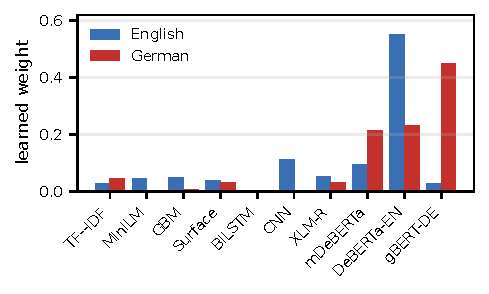
\includegraphics[width=0.92\linewidth]{figs/perlang_weights}
\caption{Per-language weights (full-fit on val). DeBERTa-v3-large EN
dominates the English mix ($0.553$) and gBERT-large DE the German
($0.448$); B4 (BiLSTM) and B2 receive zero weight on both languages.}
\label{fig:perlang-weights}
\end{figure}

On EN, DeBERTa-EN takes the largest share ($0.553$); B3 (CNN) and
mDeBERTa supply diversifying contributions ($0.113$, $0.094$). On DE,
gBERT-DE leads ($0.448$) and mDeBERTa is a strong second ($0.212$);
DeBERTa-EN still receives $0.231$ because on $\mathrm{val}_{\textsc{de}}$
it has the lowest pairwise error overlap with mDeBERTa among the
strong models (Jaccard $0.60$, vs.\
gBERT$\,\leftrightarrow\,$mDeBERTa $0.68$ and
XLM-R$\,\leftrightarrow\,$mDeBERTa $0.68$ on the same subset), and so
reduces the combined MAE. B4 (BiLSTM) and B2 are zero on both
languages---redundant given the rest of the pool.

\subsection{Error Geometry}

\begin{figure}[t]
\centering
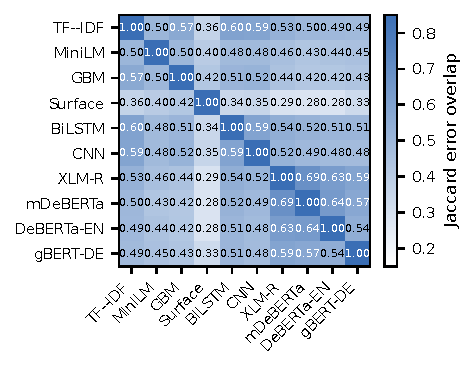
\includegraphics[width=0.92\linewidth]{figs/error_correlation}
\caption{Pairwise Jaccard overlap of error-sets on validation. The
four fine-tuned transformers form a high-overlap block
($0.55$--$0.69$); B6 (surface) is the most decorrelated from the
strong models, but at $0.72$ MAE-score its independent signal is too
weak to lift the ensemble.}
\label{fig:errcorr}
\end{figure}

The bottom-right block of \cref{fig:errcorr} confirms that the
transformer pool is highly correlated:
XLM-R$\,\leftrightarrow\,$mDeBERTa overlap at $0.69$, and the
specialists at $0.55$--$0.64$ with each other and with the
multilingual encoders. This explains the empirical ceiling: even with
ten models, the ensemble gain over the best single model is bounded
by what \emph{independent} predictors could add, and the lexical
baselines (B1, B5) do not provide enough independent signal.

\subsection{Per-Language Confusion and Progression}

\begin{figure}[t]
\centering
\subfigure[Per-language confusion.\label{fig:confpl}]{
  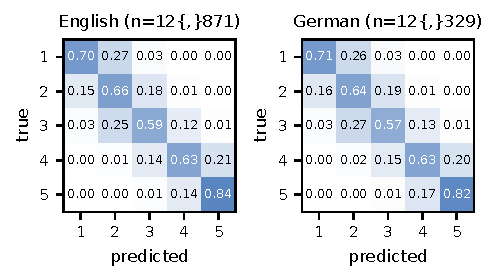
\includegraphics[width=0.55\linewidth]{figs/confusion_per_lang}}
\hfill
\subfigure[Progression.\label{fig:prog}]{
  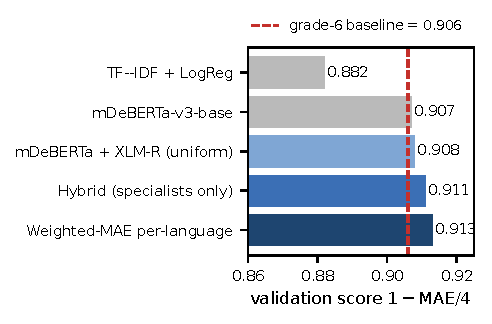
\includegraphics[width=0.40\linewidth]{figs/progression}}
\caption{(a) Row-normalised confusion matrices of the per-language
weighted-MAE ensemble; off-diagonal mass concentrates on neighbours
and the extreme $0\!\leftrightarrow\!4$ confusion stays below $0.5\%$
in both languages. (b) Validation score across the five conceptual
stages, with the grade-6 baseline ($0.906$) marked.}
\end{figure}

\cref{fig:confpl} shows the per-language confusion matrices of the
final ensemble. The diagonal is dominant in both languages; off-by-one
errors account for the bulk of mistakes; the costly
$0\!\leftrightarrow\!4$ confusion stays below $0.5\%$ on each
side---the regime MAE rewards. \cref{fig:prog} traces the score from
TF--IDF+LogReg ($0.882$) through mDeBERTa ($0.907$),
XLM-R$+$mDeBERTa uniform ($0.908$), the specialists-only hybrid
($0.911$), to the final per-language weighted-MAE ensemble ($0.913$).

% =================================================================
\section{Discussion}
\label{sec:discussion}
% =================================================================

\paragraph{Three sources of gain, of unequal size.}
Going from the strongest multilingual single model ($0.907$ on val,
$0.906$ on LB) to the final per-language ensemble ($0.913$/$0.911$)
is the cumulative effect of three additions: median decoding
($+\,$small on every model), the specialists ($+0.004$ on val,
$+0.004$ on LB, comparing mDeBERTa to the simple
specialists-only hybrid), and the per-language weighting on top
($+0.002$ on val, $+0.001$ on LB, comparing the hybrid to the final
ensemble). The specialists make the biggest \emph{single} contribution
because the multilingual encoders dilute their parameters over $100$
languages \cite{conneau2020xlmr}, while the specialists concentrate
them on one.

\paragraph{Why the gating MLP underperforms.}
The soft-routing MLP scores $0.0049$ below the per-language hard
router (\cref{tab:meta}). Its input (MiniLM embedding, per-model
uncertainties, language flag) is a superset of the hard router's; the
gap reflects the sample-efficiency tax of $\approx 26$k parameters on
$25$k samples, even with dropout $0.5$ and three-seed averaging---an
observed routing variable beats a learnt one in this regime.

\paragraph{Limitations.}
Bootstrap resampling ($10{,}000$ replicates) on the ensemble gives a
$95\%$ CI of $[0.9115,0.9148]$, above $0.906$ but narrower than
cross-validation across training seeds would yield. Reviews ambiguous
for the language rule (very short, code-switched, numeric-only) are
routed suboptimally; this is the floor on any
language-conditioned method on this corpus.

% =================================================================
\section{Conclusion}
% =================================================================

We described a pipeline for bilingual ordinal sentiment classification
that exploits two structural properties: MAE-optimal median decoding
and a per-language weighted-MAE meta-learner combining two monolingual
specialists with a pool of multilingual transformers and classical
baselines. The system scores $0.911$ on the public Kaggle leaderboard
(rank $2/27$), $+0.005$ above the grade-6 baseline. All experiments
are reproducible from the cached per-model probability arrays.

\section*{Declaration of Originality}

This project is our own work. The pre-trained models we
used---xlm-roberta-base, microsoft/mdeberta-v3-base,
microsoft/deberta-v3-large, deepset/gbert-large, and
paraphrase-multilingual-MiniLM-L12-v2---are publicly available on the
Hugging Face Hub. We did not use any external dataset, did not call any
external API for inference or generation, and did not import any
solution from previous years. All implementation relies on
\texttt{scikit-learn}, \texttt{PyTorch}, the Hugging Face
\texttt{transformers} library \cite{wolf2020transformers}, and standard
Python scientific packages.

\bibliography{report}
\bibliographystyle{icml2024}

\end{document}
